\documentclass[10pt,fleqn]{article}
\usepackage{hyperref}
\usepackage{graphicx}


\setlength{\topmargin}{-.75in}
\addtolength{\textheight}{2.00in}
\setlength{\oddsidemargin}{.00in}
\addtolength{\textwidth}{.75in}

\nofiles

\pagestyle{empty}

\setlength{\parindent}{0in}

% new math commands


\setlength{\oddsidemargin}{-0.25in}
\setlength{\evensidemargin}{-0.25in}
\setlength{\textwidth}{6.75in}
\setlength{\headheight}{0.0in}
\setlength{\topmargin}{-0.25in}
\setlength{\textheight}{9.00in}

\makeindex

\usepackage{mathrsfs}

%\usepackage[pdftex]{graphicx}
\usepackage{epstopdf}

\newcounter{beans}

\newcommand{\ds}{\displaystyle}
\newcommand{\limit}[2]{\displaystyle\lim_{#1\to#2}}

\newcommand{\binomial}[2]{\ \left( \begin{array}{c}
                                  #1 \\
                                  #2
                                 \end{array}
                            \right) \
                         }
\newcommand{\ExampleRule}[2]
  {
  \noindent
  \rule{\linewidth}{1pt}
  \begin{example}
    #1
    \label{#2}
  \end{example}
  \rule{\linewidth}{1pt}
  \vskip0.125in
  }

\newcommand{\defbox}[1]
  {
   \ \\
   \noindent
   \setlength\fboxrule{1pt}
   \fbox{
        \begin{minipage}{6.5in}
          #1
        \end{minipage}
        }
   \ \\
  }
\newcommand{\verysmallworkbox}[1]
  {
   \ \\
   \noindent
   \setlength\fboxrule{1pt}
   \fbox{
        \begin{minipage}{6.5in}
           #1
           \ \\
           \vskip0.5in \ \\
           \ \\
        \end{minipage}
        }
   \ \\
  }
\newcommand{\smallworkbox}[1]
  {
   \ \\
   \noindent
   \setlength\fboxrule{1pt}
   \fbox{
        \begin{minipage}{6.5in}
           #1
           \ \\
           \vskip2.5in \ \\
           \ \\
        \end{minipage}
        }
   \ \\
  }
\newcommand{\halfworkbox}[1]
  {
   \ \\
   \noindent
   \setlength\fboxrule{1pt}
   \fbox{
        \begin{minipage}{6.5in}
           #1 \hfill
           \ \\
           \vskip3.25in \ \\
           \ \\
        \end{minipage}
        }
   \ \\
  }
\newcommand{\largeworkbox}[1]
  {
   \ \\
   \noindent
   \setlength\fboxrule{1pt}
   \fbox{
        \begin{minipage}{6.5in}
           #1
           \ \\
           \vskip7.5in \ \\
           \ \\
        \end{minipage}
        }
   \ \\
  }
\newcommand{\flexworkbox}[2]
  {
   \ \\
   \noindent
   \setlength\fboxrule{1pt}
   \fbox{
        \begin{minipage}{6.5in}
           #1
           \ \\

           \vskip#2 \ \\
           \ \\
        \end{minipage}
        }
   \ \\
  }


% symbols for sets of numbers

\newcommand{\natnumb}{$\cal N$}
\newcommand{\whonumb}{$\cal W$}
\newcommand{\intnumb}{$\cal Z$}
\newcommand{\ratnumb}{$\cal Q$}
\newcommand{\irrnumb}{$\cal I$}
\newcommand{\realnumb}{$\cal R$}
\newcommand{\cmplxnumb}{$\cal C$}

% misc. commands

\newcommand{\mma}{{\it Mathematica}}
\newcommand{\sech}{\mbox{ sech}}
 
\newtheorem{theorem}{Theorem}
\newtheorem{example}{Example}
\newtheorem{definition}{Definition}
\newtheorem{problem}{Problem}

\setcounter{secnumdepth}{2}
\setcounter{tocdepth}{4}


\begin{document}
%%%%%%%%%%%%%%%%%%%%%%%%%%%%%%%%%%%%%%%%%%%%%%%%%%%%%%%%%%%%%%%%%%%%%%%%%%%%%%%%
%%%%%%%%%%%%%%%%%%%%%%%%%%%%%%%%%%%%%%%%%%%%%%%%%%%%%%%%%%%%%%%%%%%%%%%%%%%%%%%%
\vskip0.1in\hrule\vskip0.1in \noindent
{\bf Math 4610 Fundamentals of Computational Mathematics  - Topic 10.}
\vskip0.1in\hrule\vskip0.1in \noindent
It is very important as a computational mathematician that we use computational
resources to visualize data or output from simulations. This means producing
graphics codes that can display output from data sets in real world problems or
from computer codes that simulate real world problems. We could go back to basic
principles and write software from scratch, say using Open Graphics Library
(OpenGL) or some other set of libraries. This is time consuming and is basically
a digital exercise in reinventing the wheel.

At least initially, we should take advantage of the many software packages and
codes that produce graphics. The idea in this section of the course is to come
up with a way to display 2-d graphical output. For example, we may want to graph
a set of ordered pairs that represent data or output of a simulation. We will
have plenty of examples and problems in this course that will be aided by having
a code that will do some simple graphs of functions and/or data.

Note that there are a lot of other graphical representations of data that we
could consider. For example, surfaces, barcharts, contours and level sets, and
beyond. In this first shot a displaying graphics, we will stick to the simplest
ideas and produce a Python module/script that will produce 2D graphics. The code
will become useful in all kinds of applications, from plotting the error in 
approximations to solutions of differential equations. We will reuse the code in
some form or another throughout the semester.
%%%%%%%%%%%%%%%%%%%%%%%%%%%%%%%%%%%%%%%%%%%%%%%%%%%%%%%%%%%%%%%%%%%%%%%%%%%%%%%%
%%%%%%%%%%%%%%%%%%%%%%%%%%%%%%%%%%%%%%%%%%%%%%%%%%%%%%%%%%%%%%%%%%%%%%%%%%%%%%%%
\vskip0.1in\hrule\vskip0.1in\noindent
{\bf Visualizing Results: 2D Plotting} 
\vskip0.1in\hrule\vskip0.1in\noindent
We can start in several places, but the ideas are all centered around plotting
points in the plane and connecting the plotted points with curves of some kind
to display the behavior of an underlying function. It should be noted that no
matter how accurate the graph is, there will always be some error due to
screen resolution and finite precision in the representation of numbers. So,
suppose that we have generated a list of ordered pairs and want to plot these
values.

As an example, the content in \href{../../topic_09/html/topic_09.html}{Topic 09}
includes a couple of 2-d plots displaying the behavior of the error in
approximating a derivative with a difference quotient. In that example, a source
of some bad behavior in the derivative approximation was instantly manifested in
the graph. 

In a general setting, suppose that data in the form of a set of ordered pairs is
given. That is,
\[
  f = \left\lbrace 
       (x_0, y_0), (x_1, y_1), (x_2, y_2), \ldots, (x_n, y_n)
      \right\rbrace 
\]
This is a set of \(n+1\) data points. There is a reason for starting at zero
with our indices. That will be described when we fit a polynomial through given
data points - more on this later in the semester.

Another thing to note is that we could also take a function, say
\[
   P(t) = {{400\ e^{0.2 t}}\over{1 + 3\ e^{0.2 t}}}
\]
and sample the function at a set of input values, \(t_i\), for
\(i=0,1,\ldots,n\). The function under consideration is a solution of the
logistic differential equation for population growth. Using the formula above,
we can generate a set of ordered pairs by choosing values of the input (time)
and computing values of $P(t)$ (population density). That is,
\[
  P = \left\lbrace 
       (t_0, P(t_0)), (t_1, P(t_1)), (t_2, P(t_2)), \ldots, (t_n, P(t_n))
      \right\rbrace 
\]
Now, let's figure out a way to get a simple graph of this function. A 2-d plot
of the population density above is given in the following graph.
\vfill
\begin{figure}[h]
\centering
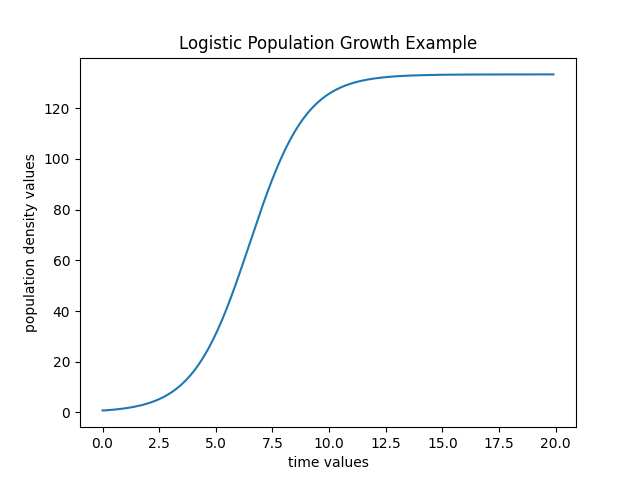
\includegraphics[width=6.0in]{../images/2dplot_01.png}
\vskip0.1in
\caption{A 2-d plot of a population density function. This is just a simple
         example of a plot that shows the results of sampling a function.}
\end{figure}
\eject
%%%%%%%%%%%%%%%%%%%%%%%%%%%%%%%%%%%%%%%%%%%%%%%%%%%%%%%%%%%%%%%%%%%%%%%%%%%%%%%%
%%%%%%%%%%%%%%%%%%%%%%%%%%%%%%%%%%%%%%%%%%%%%%%%%%%%%%%%%%%%%%%%%%%%%%%%%%%%%%%%
\vskip0.1in\hrule\vskip0.1in\noindent
{\bf Visualizing Results: 2D Plotting} 
\vskip0.1in\hrule\vskip0.1in\noindent
To create the graph shown above, a module/script was written in Python. In
addition, the development was done in an Integrated Development Environment
(IDE) named Integrated Development and Learning Environment (IDLE) that can be
used to develop bits of code into useful applications. If you have installed a
fairly recent version of Python on your computer, you should have a version of
IDLE that will come with the installation bundle. To start IDLE, you can type
\begin{verbatim}

    koebbe% idle&

\end{verbatim}
Note that there is an ampersand at the end of the command. This tells the
operating system to run the command in the background. This is a Unix feature
that allows you to run multiple processes in a single terminal.

In a terminal emulator, invoking the IDLE application looks like the window
displayed in the following figure.
\vfill
\begin{figure}[h]
\centering
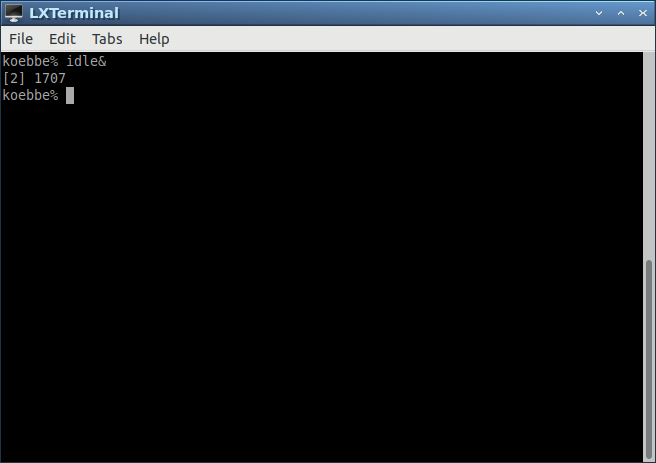
\includegraphics[width=6.0in]{../images/2dplot_02.png}
\vskip0.1in
\caption{Starting IDLE in a terminal emulator.}
\end{figure}
\eject
%%%%%%%%%%%%%%%%%%%%%%%%%%%%%%%%%%%%%%%%%%%%%%%%%%%%%%%%%%%%%%%%%%%%%%%%%%%%%%%%
%%%%%%%%%%%%%%%%%%%%%%%%%%%%%%%%%%%%%%%%%%%%%%%%%%%%%%%%%%%%%%%%%%%%%%%%%%%%%%%%
\vskip0.1in\hrule\vskip0.1in
\noindent
{\bf Opening a New File to Write Code} 
\vskip0.1in\hrule\vskip0.1in
\noindent
To get the editor up and running, you can click on the file menu in the IDLE
window and click on the New File item in the drop down menu. The window
containing IDLE will look like the next figure. 
\vskip0.1in\hrule\vskip0.1in
\vfill
\begin{figure}[h]
\centering
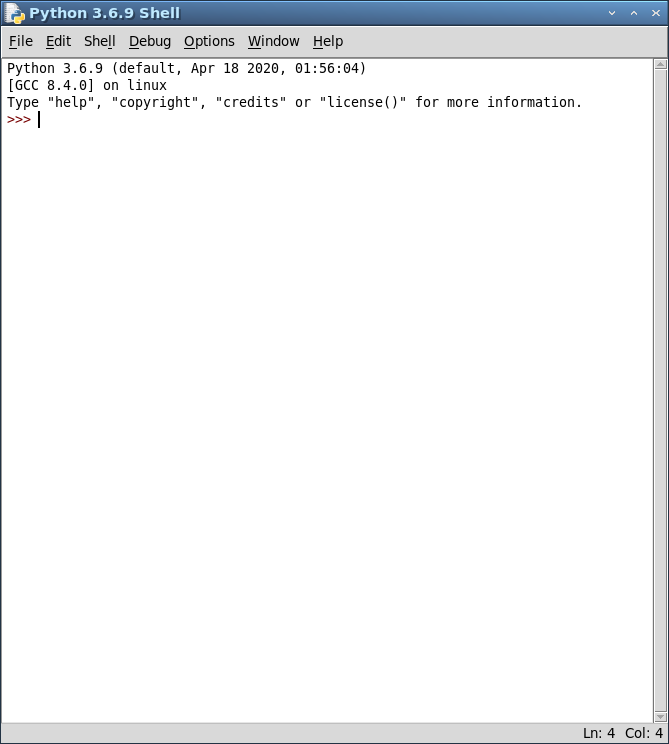
\includegraphics[width=6.0in]{../images/2dplot_03.png}
\caption{Opening a New File to write code in Python.}
\end{figure}
\eject
%%%%%%%%%%%%%%%%%%%%%%%%%%%%%%%%%%%%%%%%%%%%%%%%%%%%%%%%%%%%%%%%%%%%%%%%%%%%%%%%
%%%%%%%%%%%%%%%%%%%%%%%%%%%%%%%%%%%%%%%%%%%%%%%%%%%%%%%%%%%%%%%%%%%%%%%%%%%%%%%%
\vskip0.1in\hrule\vskip0.1in
\noindent
{\bf The Final Version of the Plotting Code in Python} 
\vskip0.1in\hrule\vskip0.1in\noindent
The next step is to type in Python code that will provide the 2-d plot that we
want.  The figure below shows the final code in the IDLE new file window. The
code can be run using the Run menu at the top of the window. When the module is
running you will be prompted to see if you want to save any changes to the code.
It is usually a good thing to save the changes.
\vskip0.1in\hrule\vskip0.1in\noindent

\begin{verbatim}

    #
    # import some stuff
    # -----------------
    #
    from matplotlib import pyplot as plt
    import numpy as np
    #
    # this is hardwired for a logistic function - so give initial time and final
    # time
    # ----
    #
    start = 0.0
    end = 20.0
    #
    # set an array of input/time values
    # ---------------------------------
    #
    t = []
    #
    # initialize a variable to keep track of the time at each iteration and append
    # the initial value to the array
    # ------------------------------
    #
    x = 0.0
    t.append(x)
    #
    # compute the time increment between samples
    # ------------------------------------------
    #
    dx = ( end - start ) / 201.
    #
    # set the functional form for the logistic solution
    # -------------------------------------------------
    #
    expression  = '(400.0 * np.exp(0.8*x)) / (500.0 + 3.0 * np.exp(0.8*x) )'
    #
    # initialize an array for the output/population density values
    # ------------------------------------------------------------
    #
    p = []
    p.append(eval(expression))
    #
    # set the loop iterator and start the while loop
    # ----------------------------------------------
    #
    l = 0
    while l < 200:
        #
        # compute the current value of the expression
        # -------------------------------------------
        #
        p.append(eval(expression))
        #
        # move on to the next value of the input
        # --------------------------------------
        #
        x = x + dx
        #
        # append the new value to the input array
        # ---------------------------------------
        #
        t.append(x)
        #
        # plus one the iterator
        # ---------------------
        #
        l += 1
    #
    # do the plot thing in matplotpy
    # ------------------------------
    #
    plt.xlabel('time values')
    plt.ylabel('population density values')
    plt.title('Logistic Population Growth Example')
    plt.plot(t, p)
    plt.show()

\end{verbatim}
\vskip0.1in\hrule\vskip0.1in\noindent
The code can be copied from these lecture notes and saved into a file. The
Python code is a hardwired version to graph the single expression
\begin{verbatim}

    expression  = '(400.0 * np.exp(0.8*x)) / (500.0 + 3.0 * np.exp(0.8*x) )'

\end{verbatim}
in python. It might be a good idea to write a general code. This will be done
in the next topic.
\vfill
\begin{figure}[h]
\centering
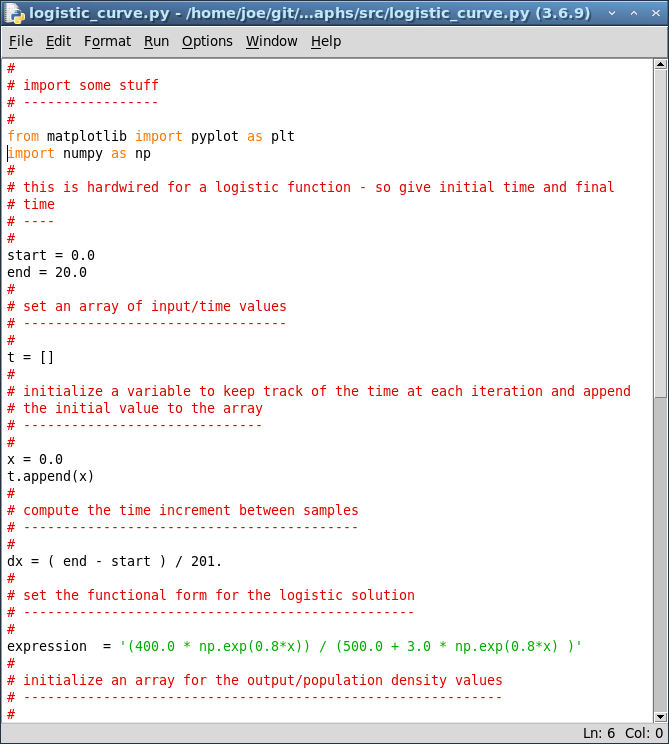
\includegraphics[width=6.0in]{../images/2dplot_05.png}
\caption{The final code in the window to produce a 2d-plot of a logistic
         population model.}
\end{figure}
\eject
%%%%%%%%%%%%%%%%%%%%%%%%%%%%%%%%%%%%%%%%%%%%%%%%%%%%%%%%%%%%%%%%%%%%%%%%%%%%%%%%
%%%%%%%%%%%%%%%%%%%%%%%%%%%%%%%%%%%%%%%%%%%%%%%%%%%%%%%%%%%%%%%%%%%%%%%%%%%%%%%%
\vskip0.1in\hrule\vskip0.1in\noindent
{\bf The Final Result} 
\vskip0.1in\hrule\vskip0.1in\noindent
When the Run menu item is selected, the result will be a new window popping up
that displays the graph in the first figure of this section of the notes.
The nice thing is that you can save a copy of the figure in several formats.
Your instructor usually likes a Portable Network Graphics (png) format. 
\vskip0.1in\hrule\vskip0.1in
\vfill
\begin{figure}[h]
\centering
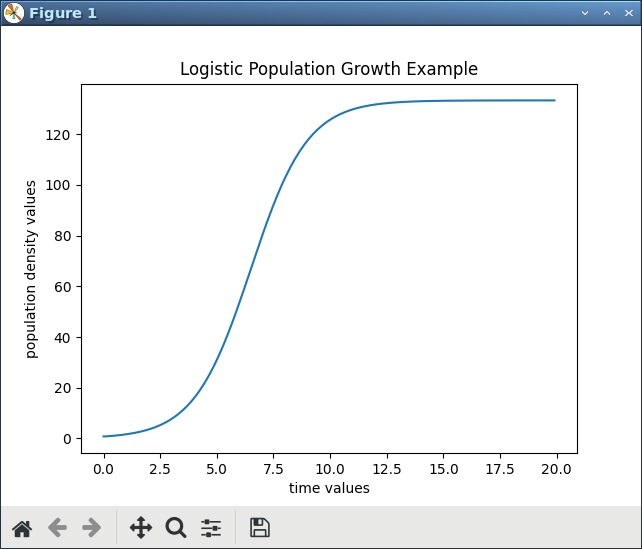
\includegraphics[width=6.0in]{../images/2dplot_06.png}
\caption{The output from the 2d plotting script is a window that shows the plot
         with a toolbar at the bottom of the window. The controls on the
         toolbar can be used to save a copy among other options.}
\end{figure}
\eject
%%%%%%%%%%%%%%%%%%%%%%%%%%%%%%%%%%%%%%%%%%%%%%%%%%%%%%%%%%%%%%%%%%%%%%%%%%%%%%%%
%%%%%%%%%%%%%%%%%%%%%%%%%%%%%%%%%%%%%%%%%%%%%%%%%%%%%%%%%%%%%%%%%%%%%%%%%%%%%%%%
\vskip0.1in\hrule\vskip0.1in \noindent
  \href{../../topic_09/md/topic_09.md}{Previous} |
  \href{../../toc/md/topic_toc.md}{Table of Contents} |
  \href{../../topic_11/md/topic_11.md}{Next}
\vskip0.1in\hrule\vskip0.1in \noindent
%%%%%%%%%%%%%%%%%%%%%%%%%%%%%%%%%%%%%%%%%%%%%%%%%%%%%%%%%%%%%%%%%%%%%%%%%%%%%%%%
%%%%%%%%%%%%%%%%%%%%%%%%%%%%%%%%%%%%%%%%%%%%%%%%%%%%%%%%%%%%%%%%%%%%%%%%%%%%%%%%
\end{document} 
